\documentclass[10pt,a4paper]{article}
\usepackage[margin=2cm, left=1.5cm, right=1.5cm]{geometry}
\usepackage{amsmath, amssymb, amsthm}
\usepackage{fancyhdr}
\usepackage{mdframed}
\usepackage{enumerate}
\usepackage{graphicx}
\usepackage{float}
\usepackage{array}
\usepackage{diagbox}
\usepackage{makecell}

\pagestyle{fancy}
\fancyhf{}
\fancyhead[L]{113-1 Machine Learning}
\fancyhead[R]{Final Project}
\fancyfoot[C]{\thepage}
\setlength{\headheight}{15pt}

\usepackage{silence}
\WarningFilter{latexfont}{Font shape}
\WarningFilter{latexfont}{Some font shapes were not available}

\usepackage{xeCJK}
\setCJKmainfont[AutoFakeBold=true, AutoFakeSlant=true]{bkai00mp.ttf}
\setCJKmonofont[AutoFakeBold=true, AutoFakeSlant=true]{bkai00mp.ttf}
\setCJKsansfont[AutoFakeBold=true, AutoFakeSlant=true]{bkai00mp.ttf}

% remove all figures for faster compilation
% \usepackage[allfiguresdraft]{draftfigure}

\linespread{1.25}

\begin{document}
\begin{center}
  {\LARGE \bf HTML 2024 Final Project}\\[8pt]
  \textbf{Team:} How To Make Lasagna\\
  B12902119 胡祐誠
  B12902123 常洧丞
  B12902037 張聲元
  B11902139 洪佑全
\end{center}


\section{Introduction}
We are running out of space just skip this part.

\section{Preprocessing}
\subsection{empty data filling}
From the dataset obtained, there are $5\%$ per column of data missing, which increases the hardness to predict and to feed the data into model.
First, there are only $30$ teams it is plausible to convert to either a one hot vector of size $30$ or floating point numbers indicating team winning probabilities.
For those empty values, we can set those empty values to $0$, or use auto encoder to fill the holes.

Since mapping all empty values to zero values is naive yet it intuitivem, which the performance lingers about $54\%$ to $57\%$.
The mapping to zero may contain large bias to the original data by $5\%$ of data are marked affect the aggregation of data.

We utilize the features of the auto encoder to rebuild the same data out of the extracted features, we can utilize it to generate data with no holes.
By auto encoder, we finally passed the baseline by simple DNN, which shows that mapping empty values to zero decreases the statistical meaning and model performance significantly.

A data too complex or having too many similar features distracts the model while training and often leads to overfitting or falling into local minima.
To solve the problem we use PCA on highly similar columns to reduces the complexity of training data by half.
Our method first finds all pair of Pearson corelation coefficients and perform disjoint set union on those pair of correlation coefficient absolute value higher than $0.5$.
Then, apply PCA on those set having element greater than 1, reduce their dimensions by half, then rebuild the data with PCA processed columns.
By doing such preprocess, we find out interesting pattern in the dataset.
Some of the data pairs are highly similar in a third rank polynomial pattern, shown as below figure \ref{fig:51-53} and figure \ref{fig:51-53r}.
We can find out that zero mapping highly distracts the dataset by forming two protruding straight lines as in figure \ref{fig:29-129} and figure \ref{fig:51-53}.
Also, from the recovered data using auto encoder, we can eliminate the two perpendicular straight lines and results in a higher $r^2$ value in the same similar pair as in figure \ref{fig:29-129r} and figure \ref{fig:51-53r}.
However, auto encoder sometimes fails to fill the accurate data and leads to some data points very far away from the data cluster as in figure \ref{fig:51-53r} the left and right most points.
After running the disjoint set union, we find out that there are $17$ goups of data to perform PCA, while two of the set has element over $10$ while others only has about $2$ to $4$ elements.
Implying the dataset has numerous similar data columns may cause distract training and lower performance.
\begin{figure}[ht]
    \centering
    \begin{minipage}{.2\textwidth}
        \centering
        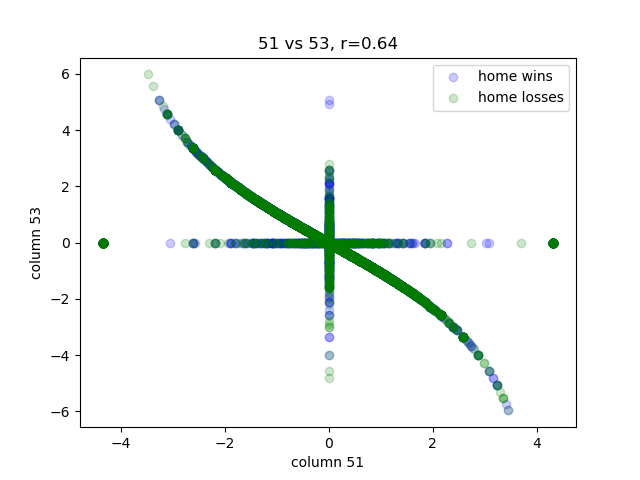
\includegraphics[width=0.8\linewidth]{images/0.64r_51_to_53.png}
        \caption[width=0.8\linewidth]{Column 51 to column 53 fill nan with zeros}
        \label{fig:51-53}
    \end{minipage}%
    \begin{minipage}{.05\textwidth}
        \ 
    \end{minipage}%
    \begin{minipage}{.2\textwidth}
        \centering
        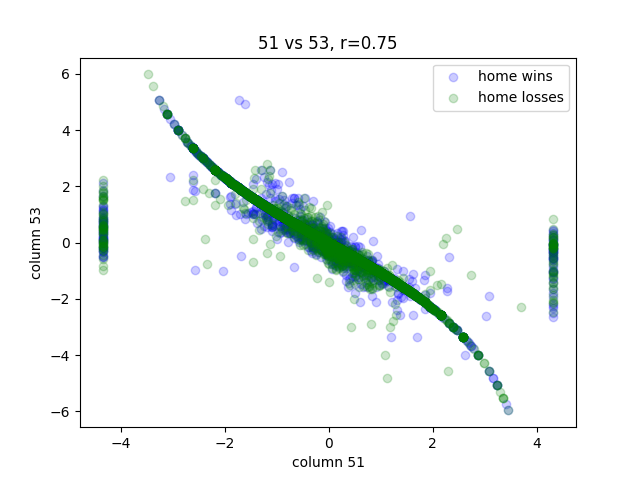
\includegraphics[width=0.8\linewidth]{images/0.75r_51_to_53_recovered.png}
        \caption[width=0.8\linewidth]{Column 51 to column 53 preprocess using auto encoder}
        \label{fig:51-53r}
    \end{minipage}%
    \begin{minipage}{.05\textwidth}
        \ 
    \end{minipage}%
    \begin{minipage}{.2\textwidth}
        \centering
        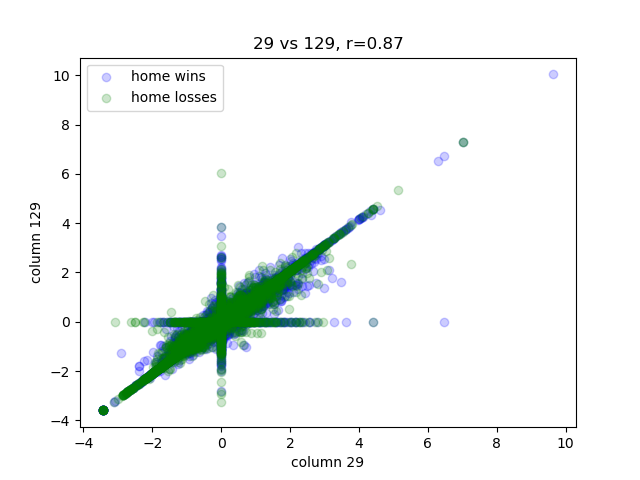
\includegraphics[width=0.8\linewidth]{images/0.87r_29_to_129.png}
        \caption[width=0.8\linewidth]{Column 29 to column 129 fill nan with zeros}
        \label{fig:29-129}
    \end{minipage}%
    \begin{minipage}{.05\textwidth}
        \ 
    \end{minipage}%
    \begin{minipage}{.2\textwidth}
        \centering
        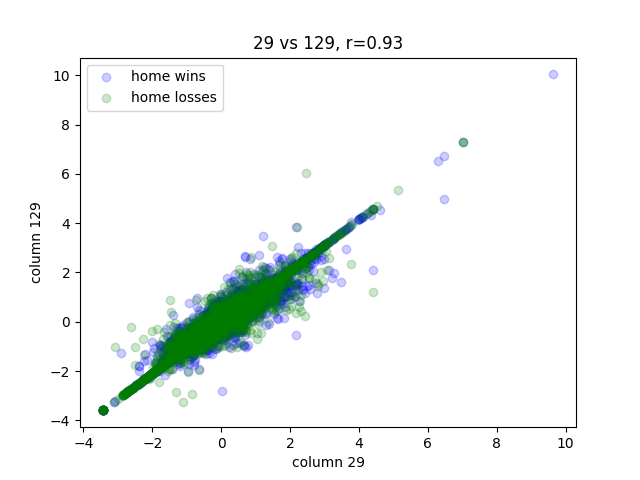
\includegraphics[width=0.8\linewidth]{images/0.93r_29_to_129_recovered.png}
        \caption[width=0.8\linewidth]{Column 29 to column 129 preprocess using auto encoder}
        \label{fig:29-129r}
    \end{minipage}
\end{figure}




\section{Model}

\subsection{Logistic Regression}
We expect that it will be the least accurate one, but we still want to see how it performs.
We used the preprocessed data to train the model, and split the data into 80\% training and 20\% validation.
We trained the model 5000 times and choose the one with the highest validation accuracy for both stage 1 and stage 2.
The highest validation accuracy we got in stage 1 was 0.64, and in stage 2 was 0.61.
In spite of this, the performance of logistic regression in private was 0.56 in stage 1, and 0.53 in stage 2.
Overall, logistic regression is one of the worst models we used in this project.



\subsection{Support Vector Machine}

Support Vector Machine (SVM) is a powerful supervised learning algorithm that can be used for our task. In this section, we discuss the application of three different SVM models: linear kernel, polynomial kernel, and Gaussian kernel. We use the \texttt{sklearn} library to implement the SVM models and perform hyperparameter tuning to optimize their performance.

\subsubsection{Linear Kernel}
We first implemented the linear SVM model, performed grid search with 3-fold cross-validation, focusing on two key hyperparameters:

\begin{table}[H]
  \centering
  \begin{tabular}{|c|c|c|}
  \hline
  Hyperparameter & Regularization Parameter (\texttt{C}) & Tolerance for Stopping Criterion (\texttt{tol}) \\ \hline
  Values & 0.1, 1.0, 10 & 0.001, 0.0001 \\ \hline
  \end{tabular}
  \caption{Hyperparameters for linear SVM model}
\end{table}

The best hyperparameters found were \texttt{C} = 10 and \texttt{tol} = 0.001. This model was then retrained on the entire training set.

\begin{table}[H]
  \centering
  \begin{tabular}{|c|c|c|c|c|c|}
  \hline
  Sample & Validation & Stage 1 Public & Stage 1 Private & Stage 2 Public & Stage 2 Private \\ \hline
  Accuracy (\%) & 63.32 & 55.68 & 55.30 & 51.41 & 52.61 \\ \hline
  \end{tabular}
  \caption{Accuracy of the best linear SVM model}
\end{table}


\subsubsection{Polynomial Kernel}
We experimented with a polynomial kernel SVM, but the results were suboptimal, yielding poor accuracy compared to the linear and Gaussian kernels. Due to its underperformance, the polynomial kernel was not considered for the final submission, and we proceeded directly to testing the Gaussian kernel, which showed more promise.


\subsubsection{Gaussian Kernel}
For the Gaussian kernel SVM, we also performed hyperparameter tuning using grid search with 3-fold cross-validation. The grid search focused on the following hyperparameters:

\begin{table}[H]
  \centering
  \begin{tabular}{|c|c|c|}
  \hline
  Hyperparameter & $C$ & $\gamma$ \\ \hline
  Values & 0.1, 1.0, 10 & 0.01, 0.001, 0.0001 \\ \hline
  \end{tabular}
  \caption{Hyperparameters for Gaussian SVM model}
\end{table}

The best hyperparameters found were \texttt{C} = 10 and \texttt{gamma} = 0.001. We use the best hyperparameters and full training data to train the final model.

\begin{table}[H]
  \centering
  \begin{tabular}{|c|c|c|c|c|c|}
  \hline
  Sample & Validation & Stage 1 Public & Stage 1 Private & Stage 2 Public & Stage 2 Private \\ \hline
  Accuracy (\%) & 57.01 & 56.29 & 57.30 & 55.90 & 53.02 \\ \hline
  \end{tabular}
  \caption{Accuracy of the best Gaussian SVM model}
\end{table}



\subsubsection{Discussion}

The learning curves  for the linear and Gaussian kernel SVM models provide insights into their performance.
The linear kernel SVM shows a consistent gap between the training and validation accuracy, indicating that the model may be underfitting the data.
In contrast, the Gaussian kernel SVM exhibits a smaller gap, suggesting that it may be better suited to capturing the underlying patterns in the data.
However, the slight decrease in validation accuracy with more training data in the Gaussian kernel SVM indicates that the model may still struggle with generalization to unseen data.
Further adjustments to the model or feature engineering may be necessary to improve its performance.



\begin{figure}[t]
  \centering
  \begin{minipage}{0.3\textwidth}
      \centering
      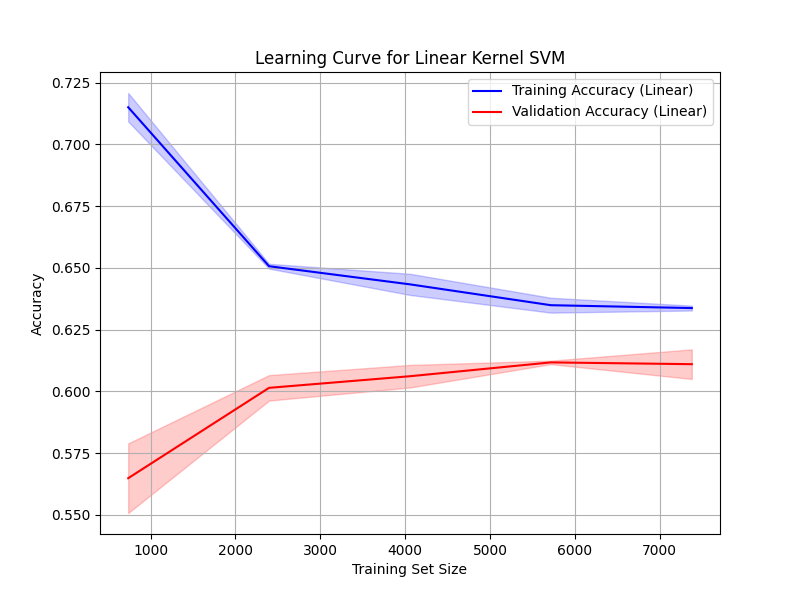
\includegraphics[width=\textwidth]{images/learning_curve_linear_SVM.png}
      \label{fig:linear_SVM_curve}
  \end{minipage}%
  \begin{minipage}{0.3\textwidth}
      \centering
      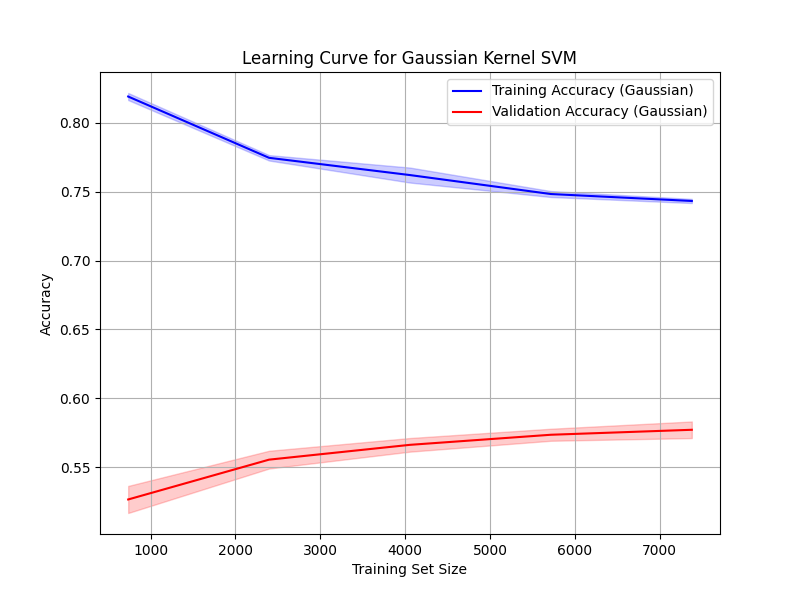
\includegraphics[width=\textwidth]{images/learning_curve_gaussian_SVM.png}
      \label{fig:gaussian_SVM_curve}
  \end{minipage}%
  \begin{minipage}{0.3\textwidth}
      \centering
      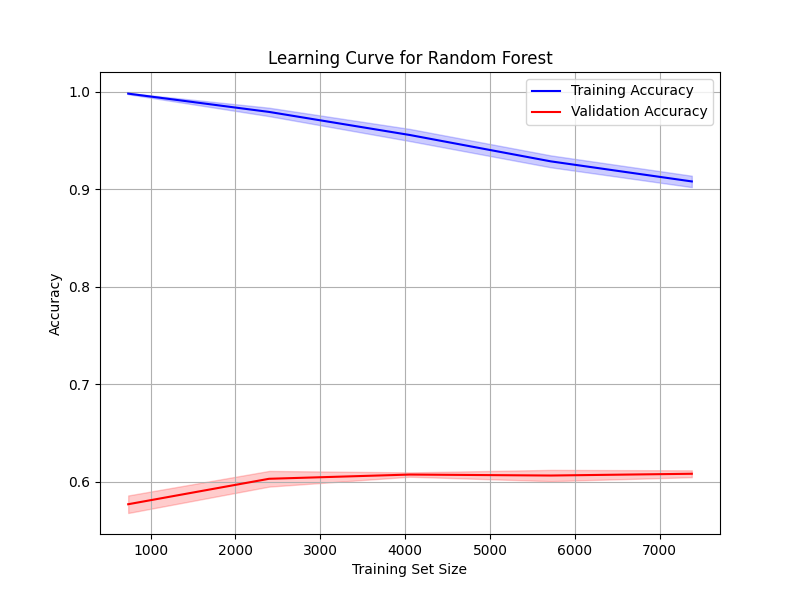
\includegraphics[width=\textwidth]{images/learning_curve_random_forest.png}
      \label{fig:random_forest_curve}
  \end{minipage}
\end{figure}



\subsection{Random Forest}

The Random Forest model was implemented using the \texttt{sklearn.ensemble.RandomForestClassifier} class, and hyperparameter tuning was performed using \texttt{GridSearchCV} with 3-fold cross-validation. The parameter grid used for tuning is shown below:

\begin{table}[H]
  \centering
  \begin{tabular}{|c|c|c|c|c|}
  \hline
  Hyperparameter & \texttt{n\_estimators} & \texttt{max\_depth} & \texttt{min\_samples\_split} & \texttt{min\_samples\_leaf} \\ \hline
  Values & 100, 200, 500, 1000 & None, 10, 20, 30 & 2, 10, 20 & 1, 5, 10 \\ \hline
  \end{tabular}
  \caption{Hyperparameters for Random Forest model}
\end{table}

Additionally, we set \texttt{max\_features} = sqrt, \texttt{bootstrap} = True, and \texttt{criterion} = gini. The best hyperparameters found during grid search were: \texttt{max\_depth} = 10, \texttt{min\_samples\_leaf} = 5, \texttt{min\_samples\_split} = 2, and \texttt{n\_estimators} = 1000. The performance are shown in the table below.

\begin{table}[H]
  \centering
  \begin{tabular}{|c|c|c|c|c|c|}
  \hline
  Sample & Validation & Stage 1 Public & Stage 1 Private & Stage 2 Public & Stage 2 Private \\ \hline
  Accuracy (\%) & 60.65 & 57.49 & 57.08 & 54.15 & 54.98 \\ \hline
  \end{tabular}
  \caption{Accuracy of the best Random Forest model}
\end{table}

The Random Forest model showed good cross-validation accuracy, but its Kaggle leaderboard performance, especially in Stage 2, was lower than expected. We anticipated better results since Random Forest can capture complex relationships and handle non-linear patterns. However, after trying various parameter settings, the performance wasn't as high as hoped. Further improvement may be possible through additional feature engineering.










\subsection{Deep Neural Network}

After trying various models, we tried to use a deep neural network (DNN). Unlike other models, DNNs do not require data preprocessing or feature transformation, which helps avoid overinterpreting the data. However, DNNs have some drawbacks: they involve many hyperparameters to tune, longer training times, and it can be difficult to find the best network structure.

The DNN model was built using Keras with TensorFlow, and hyperparameter tuning was done using 3-fold cross-validation. We tested different configurations for the network architecture, batch size, dropout rate, learning rate, and activation function. We also used early stopping with a patience of 10 epochs and reduced the learning rate if the validation loss did not improve for 5 epochs.


\begin{table}[H]
  \centering
  \begin{tabular}{|c|c|c|c|c|}
  \hline
  Hyperparameter & Batch size & Dropout rate & Learning rate & Activation function \\ \hline
  Values & 32, 64 & 0.3, 0.5 & 0.1, 0.01, 0.001 & relu, sigmoid, tanh \\ \hline
  \end{tabular}
  \caption{Hyperparameters for DNN model}
\end{table}

The best configuration found was a network with layers [128, 64, 64, 32], batch size of 64, dropout rate of 0.5, learning rate of 0.001, and activation function of tanh. This model was then retrained on the entire training set.

\begin{table}[H]
  \centering
  \begin{tabular}{|c|c|c|c|c|c|}
  \hline
  Sample & Validation & Stage 1 Public & Stage 1 Private & Stage 2 Public & Stage 2 Private \\ \hline
  Accuracy (\%) & 57.04 & 58.65 & 58.05 & 57.72 & 53.68 \\ \hline
  \end{tabular}
  \caption{Accuracy of the best DNN model}
\end{table}

The DNN exceeded our expectations, outperforming models where we spent significant time on feature engineering. Interestingly, the Kaggle score was higher than the validation score, whereas previous models typically had lower test scores. This suggests the model is not overfitting.

Dropout and early stopping helped mitigate overfitting, but the network architecture or regularization may still need improvement. Despite longer training times and complex hyperparameter tuning, the DNN's ability to learn complex patterns makes it a promising option for future work, if its complexity is properly managed.

However, the lower accuracy on the Stage 2 private leaderboard compared to Stage 1 is unexpected. This could indicate that the model doesn't generalize well to Stage 2 private data. If we emphasize the time-dependent relationships in the data, the model might perform better.





\subsection{AdaBoost}

\subsubsection{Decision Stumps}
Starting from the weakest base model, Decision Stumps. We experiment on how many decision stumps we need by 5-fold validation.
\begin{figure}[H]
  \centering
  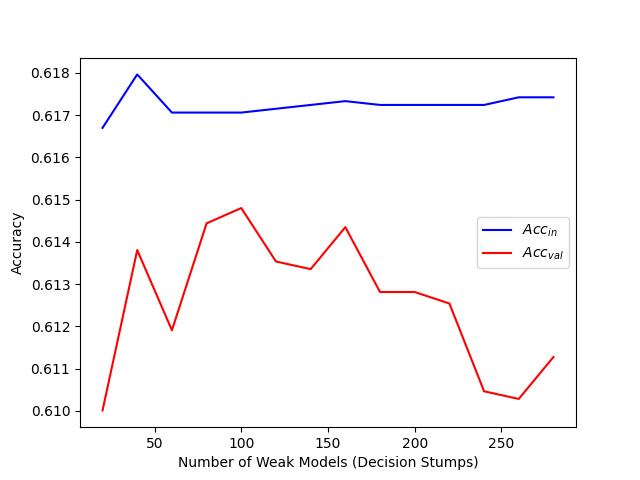
\includegraphics[width=0.2\textwidth]{images/Ada_Deci_Stump_5fold_recover.png}
  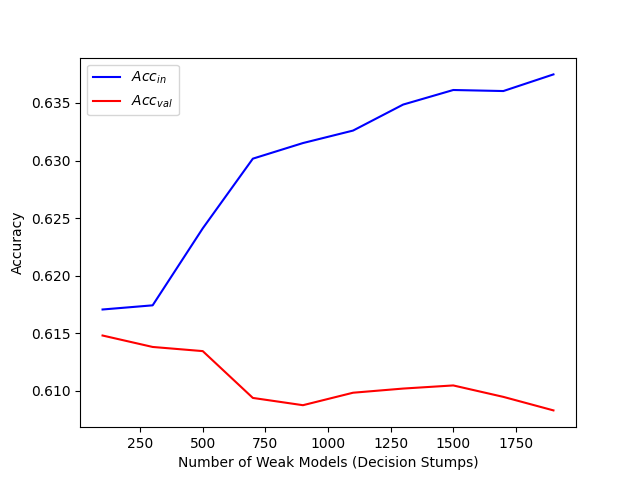
\includegraphics[width=0.2\textwidth]{images/Ada_Deci_Stump_5fold_large.png}
  \caption{Accuracy of AdaBoost with Decision Stumps}
  \label{fig:ada-deci-stump-acc}
\end{figure}
We take the best one with 100 decision stumps and get the following accuracy.
\begin{table}[H]
  \centering
  \begin{tabular}{|c|c|c|>{\centering\arraybackslash}p{2cm}|>{\centering\arraybackslash}p{2cm}|>{\centering\arraybackslash}p{2cm}|>{\centering\arraybackslash}p{2cm}|}
  \hline
  Sample & In sample & Validation & Stage 1 Public & Stage 1 Private & Stage 2 Public & Stage 2 Private \\ \hline
  Accuracy (\%) & 61.70 & 61.48 & 54.68 & 55.36 & 51.50 & 50.98 \\ \hline
  \end{tabular}
  \caption{Accuracy of AdaBoost with Decision Stumps }
  \label{tab:ada-deci-stump-acc}
\end{table}

Not very ideal, but we can do better with AdaBoost.

\subsubsection{Decision Trees}
AdaBoost can be coupled with better base learner such as shallow Decision Trees, which has way more hyperparameters to tune than Decision Stumps. To find the best model, we apply extensive Grid Search with 5-fold validation on these hyperparameters in Scikit-Learn's DecisionTreeClassifier and AdaBoostClassifier API.

\begin{table}[H]
\centering
\begin{tabular}{|c|c|c|c|c|c|}
\hline
hyperparameter & max\_depth & max\_features & min\_samples\_leaf & min\_samples\_split & n\_estimators \\ \hline
range & 2 - 10 & \{None, sqrt\} & 1 - 100 & 2 - 100 & \multicolumn{1}{c|}{20 - 200} \\ \hline
\end{tabular}
\caption{Hyperparameters for AdaBoost with Decision Trees }
\label{tab:my-table}
\end{table}
% Each of them means
% \begin{enumerate}
%     \item max\_depth: The maximum depth of the decision trees.
%     \item max\_features: The number of features to consider when looking for the best split. None means taking all $n$ features and sqrt means taking only $\sqrt{n}$ features. 
%     \item min\_samples\_leaf: The minimum number of samples required to be at a leaf node.
%     \item min\_samples\_split: The minimum number of samples required to split an internal node.
%     \item n\_estimators: The number of decision trees. 
% \end{enumerate}

Best $E_{val}$ happens around $max\_depth = 2$ or $=3$, max\_features being None, $min\_samples\_leaf=10$, $min\_samples\_split=2$ and $n\_estimators = 100$. We have the following accuracy.

\begin{table}[H]
  \centering
  \begin{tabular}{|c|c|c|>{\centering\arraybackslash}p{2cm}|>{\centering\arraybackslash}p{2cm}|>{\centering\arraybackslash}p{2cm}|>{\centering\arraybackslash}p{2cm}|}
  \hline
  Sample & In sample & Validation & Stage 1 Public & Stage 1 Private & Stage 2 Public & Stage 2 Private \\ \hline
  Accuracy (\%) & 61.95 & 62.15 & 56.16 & 55.98 & 53.65 & 53.19 \\ \hline
  \end{tabular}
  \caption{Accuracy of AdaBoost with Decision Trees }
  \label{tab:ada-deci-tree-acc}
\end{table}

We can see the improvement, but we haven't unlocked the full potential of boosting yet.

\subsection{XGBoost}
XGBoost is known as eXtreme Gradient Boosting, one of the most powerful and efficient boosting model. Most interestingly, XGBoost can be trained on raw data with missing entries, so we can compare performance on all types of preprocessing on data.

\subsubsection{Decision Trees}
XGBoost with Decision Trees has hyperparameters similar to AdaBoost's, what's interesting is that we can apply L1/L2 regularization on it. In addition, we trained XGBoost on four kinds of data, data with and without AutoEncoder filling, and data with and without PCA. 
After extensive Grid Search with 10-fold validation, we obtain the following accuracy.

\begin{table}[H]
  \centering
  \begin{tabular}{|c|c|c|c|c|c|c|}
  \hline
  \diagbox{Data}{Sample} & In sample & Validation & \makecell{Stage 1\\ Public} & \makecell{Stage 1\\ Private} & \makecell{Stage 2 \\Public} & \makecell{Stage 2\\ Private} \\ \hline
  \makecell{No PCA, filling} & 63.65 & 56.41 & 58.16 & 58.08 & 57.72 & 54.08 \\ \hline
  \makecell{No PCA, has filling} & 61.29 & 56.18 & 57.32 & 57.82 & 57.80 & 56.04 \\ \hline
  \makecell{Has PCA, no filling} & 64.94 & 62.06 & 56.13 & 56.30 & 52.74 & 52.53 \\ \hline
  \makecell{Has PCA, filling} & 64.94 & 62.06 & 56.29 & 56.23 & 52.65 & 52.36 \\ \hline
  \end{tabular}
  \caption{Accuracy (\%) of XGBoost with Decision Trees, With or Without PCA and Recovery }
  \label{tab:xgb-deci-tree-acc}
\end{table}

We can see that data with absolutely no preprocessing tends to give us a better result in both stages, public and private. It is also noticeable that data with PCA misleads us with higher validation accuracy but perform poorly on out-of-sample dataset. \\
On the other hand, AutoEncoder filling doesn't make a significant impact except on Stage 2 Private, this is possible since after all, only $5\%$ of data is missing.\\
Also, tree heights of Decision Trees differ in different kinds of boosting algorithm and datas. In AdaBoost on data with PCA, best height is around 2 and 3, but XGBoost on data with PCA, tree tends to grow to height of 9, however, XGBoost with completely raw data only needs tree with height less than 5 to achieve remarkable performance. All of them only need 50 to 100 decision trees. This can be due to the difference in boosting algorithm and variance of regularization.\\
But overall, we achieve leaps in performance with XGBoost.

% Delete for the sake of length
% \subsubsection{Dart}
% Dart is a special kind of Decision Tree model that implements dropouts which sometimes battle overfitting. It shares basically all the hyperparameters with Decision Tree so the tuning is similar. After extensive Grid Search we obtain the following result.

% \subsubsection{Linear Regression}

\subsection{Blending}
With all the various models we previously built, we can apply blending with different weight to achieve better performance. 
We apply three types of blending scheme in total, uniform, weight proportionate to model's accuracy, and weight proportionate to the triple exponential of model's accuracy. 
Since all accuracies are close to each other, weight proportionate to the accuracy can only work as tie breaker. To emphasize the opinion of the better models, we amplify the accuracy by taking the triple exponential. 
Note that the base number of the exponential needs to be chosen carefully so the blending will neither be identical to the most dominant model or the previous blending method. In Stage 1 and Stage 2 we chose 3.85 and 3.65 respectively.

\begin{table}[H]
  \centering
  \begin{tabular}{|c|c|c|c|}
  \hline
  Method & Uniform & Proportionate to acc & Proportionate to Triple Exponential \\ \hline
  Stage 1 Public & 59.07 & 59.01 & 59.46 \\ \hline
  Stage 1 Private & 57.88 & 58.08 & 57.73 \\ \hline
  Stage 2 Public & 59.22 & 59.05 & 58.72 \\ \hline
  Stage 2 Private & 53.676 & 53.92 & 54.00 \\ \hline
  \end{tabular}
  \caption{Accuracy (\%) of Blendings}
  \label{tab:blending-acc}
\end{table}

All kinds of blending performs outstandingly in Public, but all of them seriously overfit to the Public and have some disappointing Private score. 
This is possibly caused by the blunt act of blending results without validation.

\subsection{Clustering Methods}
In this project we tries to perform data splitting than assign the best arrangement of winning and losing on the data in the same cluster.
Since logistic regression, voting, DNN and most other method can be seen as seperating data points and the closest data will be assigned with the same win or lose.
Hence, we apply K-means clustering, Gaussian Mixture Model, and Mean Shift Clustering to cluster data points into different groups.
Then, we assign all groups with the $E_{in}$ maximizing output.
Hence, when prediction, the data point clustered into the specific groups will be assigned to the corresponding output identical to other data points in the same group.
In k-means clustering, the data points are cutted into $k$ groups and iterates from $2$ to $1200$.
However, when $k$ reaches $1200$ it means that every $10$ data point will be assigned to the same group where is super overfitting.
Whereas, the $E_{in}$ is still as high as $0.4$, which is unacceptable.
In GMM, we iterate $k$ from $1$ to $300$.
It performs the same as k-means clustering, but overfits much faster, about 4 times more speed.
In Mean Shift Clustering, the $k$ is optimized by the sklearn cluster model, and samely applies best assignment to each group ends up performance of $52\%$.
By the result of three clustering model, we may conclude that the dataset in this final project is low related to the relation of distance in each data point, even super overfitting do no have result greater than $70\%$ accuracy.


\section{Result}

\section{Discussion}

\section{Reference}

\end{document}
